\chapter{Introduction}
\label{chap:intro}

Data is everywhere. Our devises produce it. Our web sites consume
it. Governments collect it~\cite{GreenwaldPrism} and business request
it. But in this ever present whirlpool of data exchange, how can we
stay in control of our data? How can we ensure that those who we wish
to can access it can while preventing those who we do not from doing
the same?

Fortunately, there are methods for securing our data: strong
cryptography systems like AES or RSA are perfectly capable of allowing
us to control exactly who can read our data. Unfortunately, these
systems are often difficult if not impossible for the average end user
to employ properly. Other times, they are simply treated like ``magic
fairy dust'' to be applied to various products in the name of
``just-add-crypto'' security with little heed paid to the security of
the implementation or components of the system.

How can we make encryption more usable? How can we make it more
accessible? And how can we accomplish both while maintain capability
with an array of modern use cases involving sharing, syncing, and
growing demand? Custos aims to provide an answer to these questions by
providing a secure key-value store that can be used to implement a
key-storage as a service platform.

The work presented in this document provides the following:

\begin{packed_item}
\item An overview of the Custos architecture, rational, and design goals
\item A discussion of various use cases in which Custos can be used to
  improve security, privacy, and usability.
\item A definition of the Custos protocol and message exchange formats.
\item A prototype Custos server reference implementation.
\item Several prototype type client implementations that leverage Custos to
  add security and features not previously available.
\end{packed_item}

\section{Overview}

At it's core, Custos is just another key value store. Actually, it's
not even that. It's just a wrapper around one of several existing
key-value stores. It is not the method of key-value storage that makes
it unique. Instead, it is it's ability to provide flexible,
fine-grained access control to key-value pairs that make it
interesting. These access control capabilities make Custos an ideal
system for implementing a secure encryption key storage service. For
it is not encryption itself that leads to usability issue, but the
inadequate methods available to manage and store encryption
keys~\cite{Kher2005}. Custos aims to solve the key-storage problem
inherent in many modern applications on cryptographic security. In
doing so, it strives to enable a variety of new use cases and data
security paradigms not readily available today. In this section, we'll
discuss the basics of the Custos rational and goals.

\subsection{Separating Functionality from Trust}

Data security is an issue of trust. Who do we trust to access our
data? Who do we trust not to misuse it? Who do we trust not to share
it without permission? Today, we have very little practical ability to
make decisions regarding who we should trust with our data. Do you
want to use Facebook to communicate with family and friends? Great,
but you must trust Facebook with your personal data. Want to use Gmail
for its sleek web interface and cloud-based accessibility? Fine, but
you must trust Google with all of your email. Sure, you could forgo
Facebook or Google or any of a wide variety of web services to avoid
trusting them with you data, but as you drift toward the hermitage of
self-imposed digital exile, the last of your former friends slowly
fading from memory as they cease to even recall your existence absent
their normal methods of web based contact, fumbling through the
vestigial pages of a phone book vainly hoping to find a number for
someone's cell phone that has never, and will never, be listed there,
you may decide that giving up control over whom you trust with your
data is a perfectly fair price to pay to rejoin the 21st century land
of living, breathing, digitally exposed souls.

And even if you could live without modern cloud-based services, even
good old fashioned computing technology involves placing trust in
systems or parties beyond our control. Do you trust your computer
manufacture not to have installed a hardware key logger that sends
back data to it's parent? Do you trust your operating system not to
have a government-mandated back door for covert third party access?
Do you trust yourself not to loss your laptop, exposing all of the
data on it to whomever might find it?

\begin{figure}[!tb]
  \vspace{5ex}
  \begin{center}
    \begin{subfigure}{.32\textwidth}
      \begin{center}
        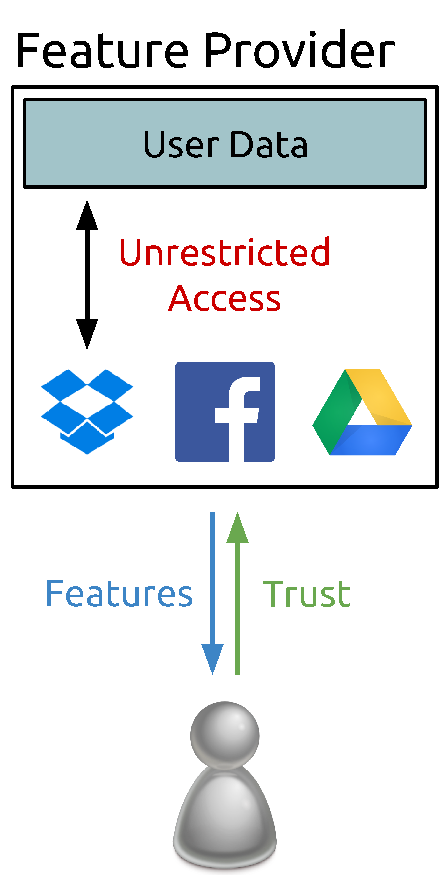
\includegraphics[height=200pt]{./figs/pdf/TrustModel-Traditional.pdf}
        \caption{Traditional}
        \label{fig:trust-traditional}
      \end{center}
    \end{subfigure}
    \begin{subfigure}{.65\textwidth}
      \begin{center}
        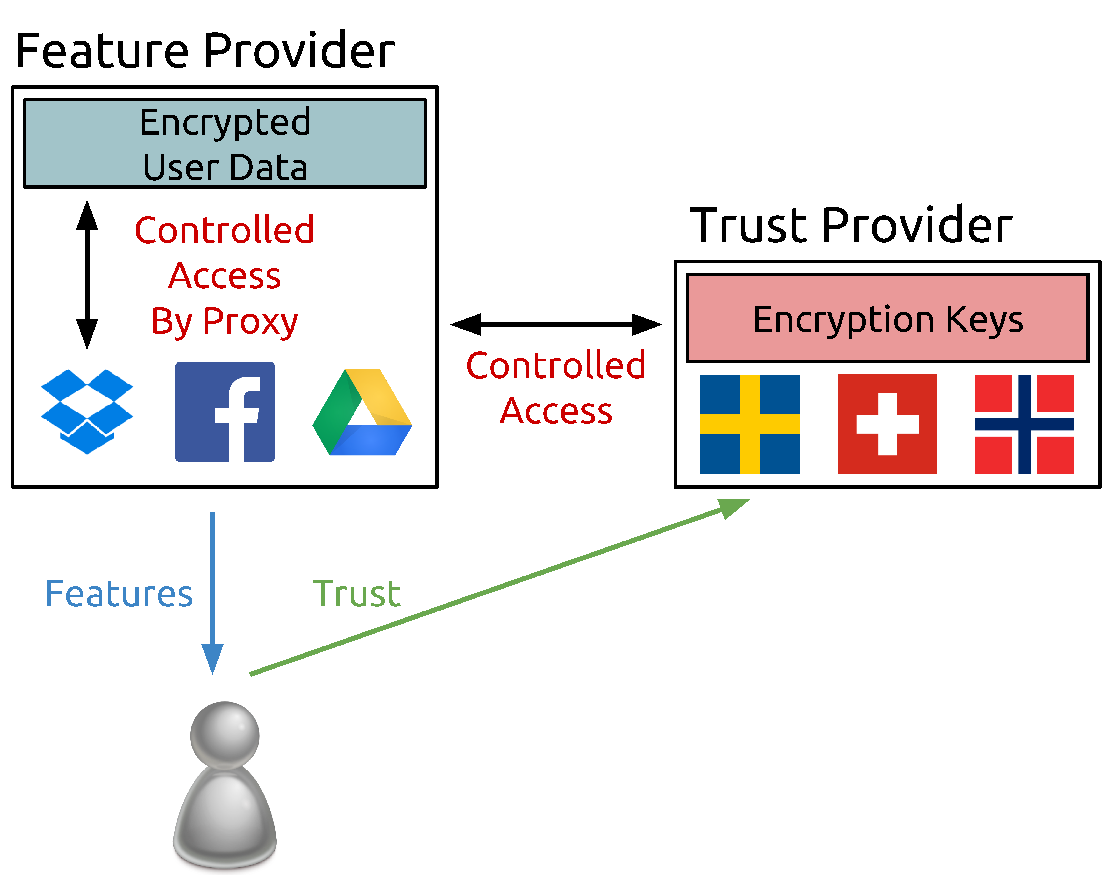
\includegraphics[height=200pt]{./figs/pdf/TrustModel-Seperated.pdf}
        \caption{Separated}
        \label{fig:trust-seperated}
      \end{center}
    \end{subfigure}
  \end{center}
  \caption{Evolving Trust Models}
  \label{fig:trust}
\end{figure}

This is the crux of the problem. In order to benefit from many of the
modern features and amenities of the digital world, you must pay the
entry price of deference of trust to organizations, technologies, and
individuals whether you would like to or not (Figure
\ref{fig:trust-traditional}).

So how can we solve this problem? This disconnect between the services
we desire and the trust we'd prefer not to cede? It seems unlikely
that we can eliminate trust form the equation all together. Systems
are too fragile and technology tied to human action; we will always
require some level of trust in some part of the system we rely on.

We might not be able to remove trust, but what if we could at least
isolate it. Separate trust from features. Disentangle what we use from
who we trust. What if we could have one company we trusted with
storing and controlling access to our data and another company we
relied on to take that data provide us with a useful service using it:
the ability to use Facebook or Google without trusting (or at least
unrestrictedly trusting) Facebook or Google (Figure
\ref{fig:trust-seperated}).

With such an ecosystem, we might be able to rely on markets or similar
means to provide us with the basic platform for securing our
data. Trustworthiness would become a service; a commodity to be bought
and sold. We could chose and pay the companies responsible for
securing our data based on their level of trustworthiness, while
choosing and paying the companies that use our data and us it provide
us with relevant features on the basis of the feature they
provide. This would remove the current coupling of features and trust
we see today, a coupling that often leads to a conflict of interest
between the features we desire and the trust we're willing to
provide. Instead we'd assign trust on the basis of perceived
trustworthiness while selecting untrusted services on the basis of
feature sets; the trusted party acting as a gatekeeper between the
untrusted party and our data. We could even distribute trust across
multiple parties to avoid having to trust any single party
completely. Such a decoupling of trust and services would provide a
lot of flexibility to maximize both the security, and the utility, of
our data.

\subsection{The Importance of Usability}

Strong encryption provides the basis for a system of separating trust
from features. With it, we can lock-down our data, rendering it
unusable to all but those to whom we grant access. Once data has been
encrypted, access to the data ciphertext itself need no longer be
granted or denied on the basis of trust. The ciphertext can be exposed
to the world confident in the knowledge that it will be indecipherably
useless without also having access to the corresponding encryption
keys. But if encryption is the lock we place on our data, then trust
becomes a matter of to whom we grant the keys. Unfortunately, while
encryption itself may be easy and well understood, securely storing,
managing, and utilizing encryption keys is hard.

It is the key management challenges that leads to many of the known
usability problems with modern encryption systems \cite{Whitten1999,
  Sweikata2009, Kher2005}. Modern encryption systems tend to be
inflexible. They force the user into a pre-defined security paradigm
and specific use case. For example, today we use systems like
Dropbox~\cite{dropbox} or Google Drive~\cite{google-drive} to store
and sync our files across a range of computers and mobile devices, but
few existing encryption schemes support this kind multi-device
access. When we wish to transfer and share files, we often do it via
e-mail attachments or removable media, but these forms of
``out-of-band'' sharing are not supported by most existing data
encryption systems. Many of our modern (and legacy) computing services
are designed to run in the background, devoid of interactive input,
but most existing encryption solutions require interactive input in
order to securely access encrypted data.

Most modern encryption systems are built around a ``one size fits
all'' mentality, leaving the user with very little flexibility to
control the manner in which their encrypted data might be used or
shared. Nor do such systems acknowledged the fact that not all
encrypted data need be protected with the same level of security. Some
data, like social security numbers, must be to be shared with a
multitude of 3rd parties. Other data, like personal photos, should be
shared, but only with specific friends or family members. Still other
data is completely private, and should never be shared at all. The
user knows how sensitive each piece of data is, and how it should be
used, but most encryption systems fail to expose a flexible method for
allowing the user to protect data on the basis of sensitivity and
desired use.

\begin{figure}[!tb]
  \vspace{5ex}
  \begin{center}
    \begin{subfigure}{\textwidth}
      \begin{center}
        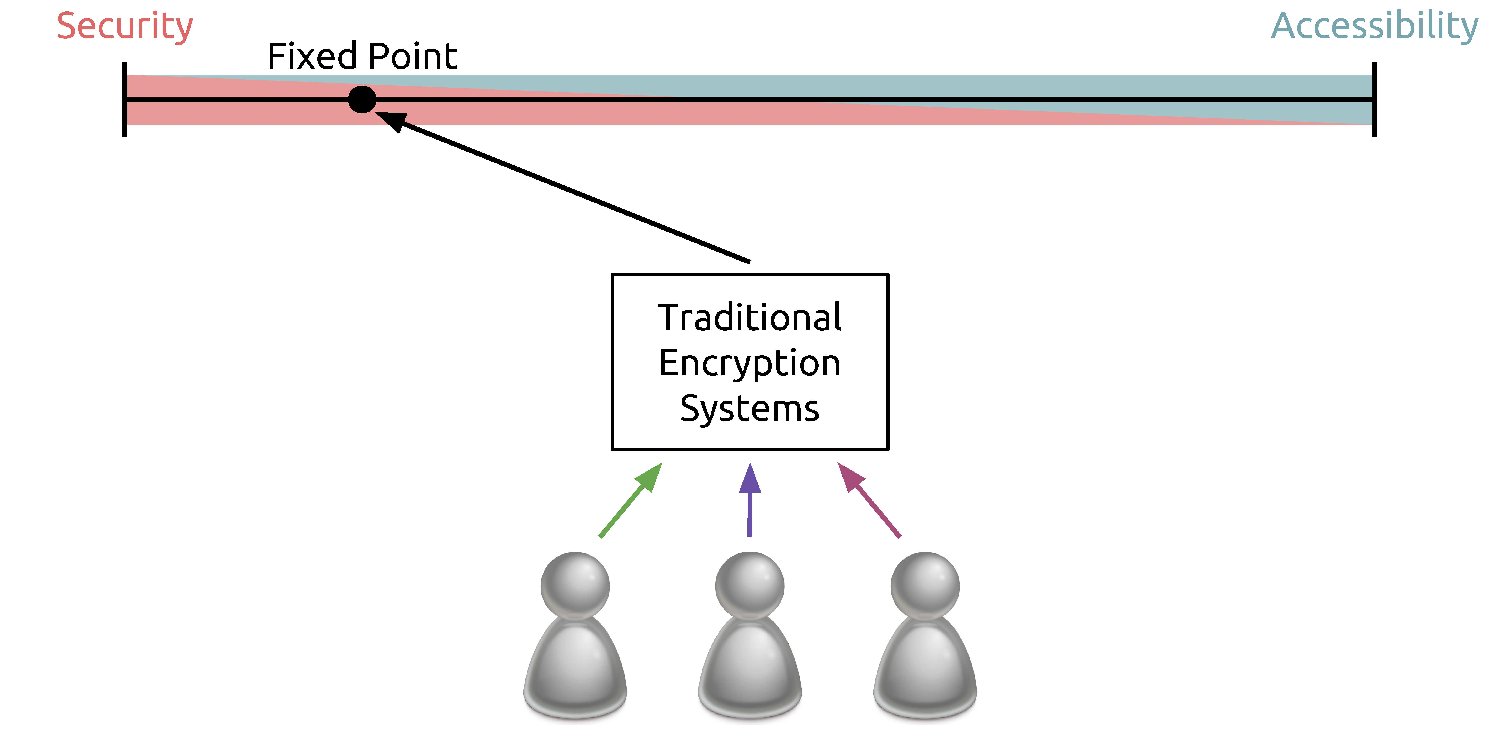
\includegraphics[height=200pt]
                        {./figs/pdf/SecuityToAccessibility-Traditional.pdf}
        \caption{Traditional}
        \label{fig:SvA-traditional}
      \end{center}
    \end{subfigure}
    \begin{subfigure}{\textwidth}
      \begin{center}
        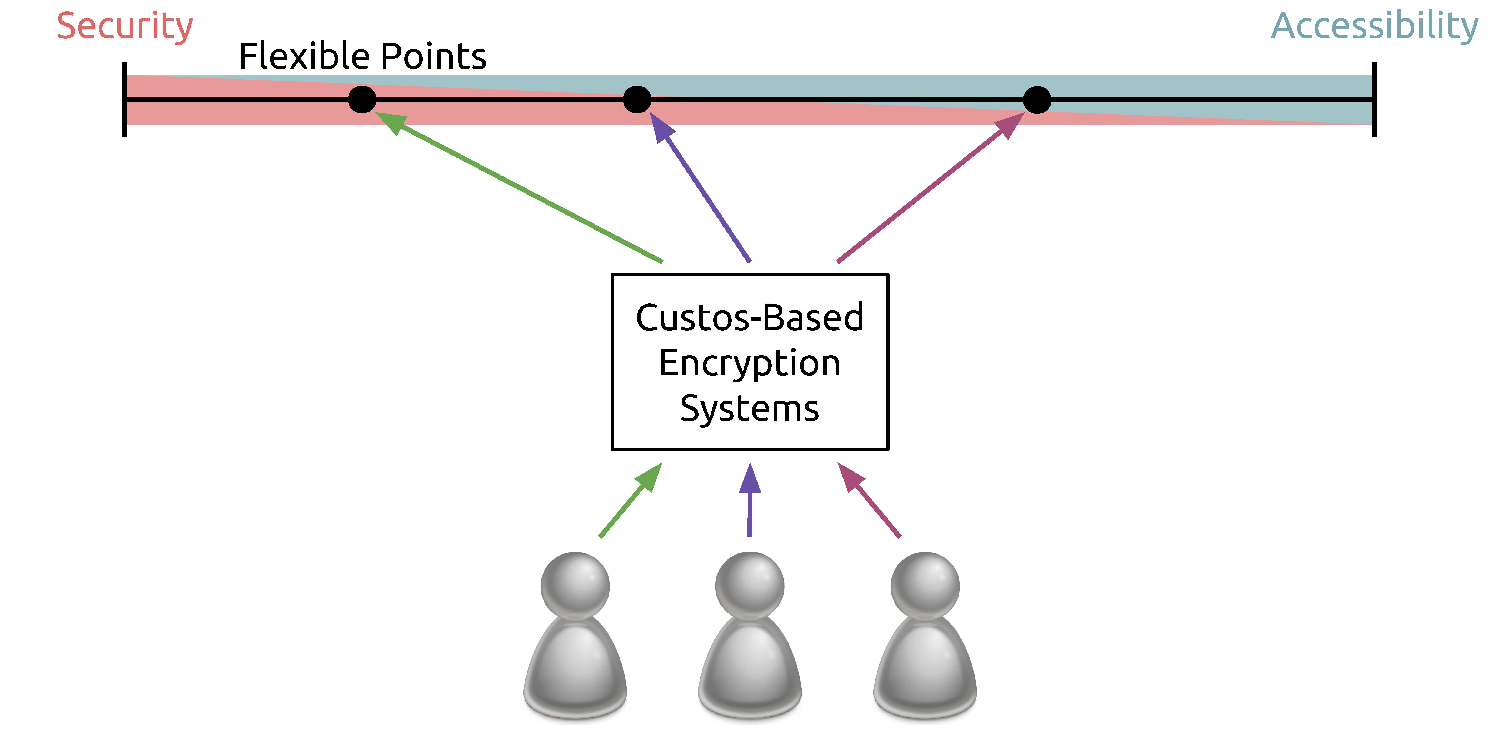
\includegraphics[height=200pt]
                        {./figs/pdf/SecuityToAccessibility-Custos.pdf}
        \caption{Custos}
        \label{fig:SvA-custos}
      \end{center}
    \end{subfigure}
  \end{center}
  \caption{Balancing Security vs Accessibility}
  \label{fig:SvA}
\end{figure}

It is often said that security and accessibility are at odds. That one
can not be improved except at the expense of the other. And that this
fact makes secure systems inherently challenging to use. While we do
not believe that security vs accessibility is truly a zero sum game,
there is some truth to the fact that security and accessibility are
often at odds. Security and accessibility exist on a continuum, with
fully accessible, minimally secure system on one side, and minimally
accessible, highly secure systems on the other. Many will say that
this inherent security vs accessibility trade-off means that secure
systems will never be easily usable. But it is not this security vs
accessibility trade-off that leads to usability issues. It is the fact
that many secure systems lock the user into a specific value on the
security vs accessibility spectrum that causes usability issues
(Figure \ref{fig:SvA-traditional}). Such inflexibility forces a user to
surmount unnecessary hurdles and forgo certain ease of access for data
that need only be minimally secure while also denying users the means
to fully secure highly sensitive data. This mismatch between user
requirements and system capabilities is a sure recipe for usability
challenges.

The inability of existing encryption systems to accommodate a diverse
range of use cases and to grant the user the flexibility to properly
place various pieces of data at various points on the security vs
accessibility spectrum leads to such systems being very difficult to
use. Fortunately, this inflexibility is not due to the underlying
encryption itself, but to the inadequate methods by which encryption
keys are managed and stored. Today, most data encryption solutions
tightly couple key storage with the underlying encryption system. This
is a mistake that has lead to a growing usability gap, and the
corresponding underutilization, of encryption as a tool for securing
and controlling our data. If encryption is going to provide a
mechanism for controlling access to our data, it needs a flexible key
storage mechanism (Figure \ref{fig:SvA-custos}).

\subsection{Key Storage as a Service}

We propose separating key storage and access management from the
underlying encryption systems through a ``Key Storage as a Service''
architecture. Such a service can make encryption systems far more
flexible and accommodating of the diversity of modern use cases, and
by extension, can make encryption far easier to use. Strong encryption
is one of the best available tools for securing and protecting our
data. We wish to reclaim it as a viable option for controlling our
data in environments that are increasingly outside of our control. We
wish to use encryption to secure our data, while designating trusted
Key Storage as a Service providers to control access to it.

In a Key Storage as a Service architecture, the underlying encryption
systems delegate key storage and access control to a separate service
instead of embedding these features directly. The key storage platform
exposes a common API, capable of being used with a variety of
encryption services. Encryption services tag encrypted data with a
unique ID, and then store this ID and the corresponding encryption key
with a key storage provider. When a system wishes to decrypt data, it
queries the key storage service for the encryption key corresponding
to the data's ID tag, and, assuming the system can satisfactorily
authenticate to the key storage service and has permission to access the
request keys, the key storage service returns the encryption key
allowing the service to decrypt the data. This separation of encryption
system and key storage allows to multiple encryption systems, or
multiple instances of an encryption system, to all access a centralized
key store. It also allows encryption systems to focus on encryption,
while key storage systems can focus of access control and auditing.

\section{Background}

Custos builds on a number of existing technologies and systems: from
basic encryption systems to distributed storage technologies to
protocol and systems design principles. In some cases these
technologies form the basis of the Custos architecture, in other,
Custos is a direct reaction to the existing limitations of these
systems. We discuss the background on which Custos is build in this
section.

\subsection{Encryption}

Modern digital encryption systems come in two flavors: symmetric and
asymmetric encryption. Symmetric encryption algorithms use the same
key to both encrypt and decrypt data. Asymmetric systems use two keys;
when one key is used to encrypt the data, the other can be used to
decrypt it, and vice versa. Both encryption systems have a place in
the modern security landscape: symmetric systems for their high
resistance to cracking and quick encrypt/decrypt performance and
asymmetric systems for their avoidance of the key exchange problem
that makes them the basis of modern public-key cryptography
technologies.

Symmetric encryption ciphers like AES (Rijndael)~\cite{Daemen1999},
Twofish~\cite{Schneier1998}, or Camellia~\cite{Matsui2004} are
well-established, fast, and secure method for encryption
data. Systematic encryption ciphers use a single key for both
encryption and decryption. This key must be securely stored, or if
shared, securely exchanged between parties. Anyone with the key can
decrypt the corresponding ciphertext the key was used to
create. Symmetric encryption systems are the preferred means of
encrypting files, hard disks, and other large chunks of data due to
their speed and relative simplicity of implementation. They tend to be
well understood, and generally considered highly secure. The security
of a symmetric encryption cipher tends to be directly related to the
length of the encryption key. Common keys lengths generally considered
secure today include 128-bit keys, 256-bit keys, and 512-bit keys.

Asymmetric encryption systems, unlike systematic encryption systems,
rely on two keys: when one key is used to encrypt the data, a second,
related key is used to decrypt the data, and vice versa. This two key
systems make asymmetric encryption systems ideal for sharing encrypted
data: one key can be publicly released, and the other is Key privately
secret. Anyone can use the public to encrypt data that only you can
decrypt using your private key. Thus, asymmetric encryption systems
like RSA~\cite{Rivest1978} form the basis for modern public-key
cryptography systems. Asymmetric ciphers tend to be slower and more
complex than symmetric ciphers. Like asymmetric ciphers, the security
of an asymmetric cipher is related to the length of the keys in a key
pair.

Often symmetric and asymmetric cryptography are used together, each
system playing to it';s straight. Symmetric ciphers are good at
quickly and securely encryption data, making them appropriate for the
core of an encryption system. Symmetric ciphers, however, suffer from
a lack of natively secure method for exchanging the required
encryption key. This is where asymmetric cryptography and related
secure key exchange systems like Diffie-Hellman~\cite{Diffie1976} come
in handy. Since they provide the basis for securely exchanging stat
over insecure channels, they can be used to exchange the symmetric
encryption key actually used to encrypt the underlying data. Such
systems are common in many modern protocols like
SSL~\cite{Freier2011}, TLS~\cite{Dierks2008}, and
OpenPGP~\cite{Callas2007, openpgp}.

Custos uses and supports a verity of the above technologies. In
general, we believe that Custos will be used to store and symmetric
encryption keys, due to symmetric ciphers core place in data
encryption. It is also symmetric keys that require the most management
since they lack a built-in secure exchange method. Custos, however,
leverages asymmetric technologies like TLS to implement the secure
exchange of the stored symmetric encryption keys and related
authentication data. Custos aims to improve upon existing systems for
managing and exchanging encrypted data (e.g. OpenPGP) by providing
more flexibility, extensible, and thus better usability than such
system normally afford.

\subsection{Human Factors}

Security research and human factors research have not always been kind
bedfellows. Fortunately, the last 15 years have seen a rise in human
factors research related to the usability of security products and
systems. This research has served to underline the growing
understanding that security without usability isn't really security at
all. If users refuse to utilize security systems because they are too
much of a burden, or if the incorrectly use them do to lack of
understanding, the security such systems provide is largely
useless. The growing awareness of usability concerns related to
security systems has led to an increased effort to build systems that
are both secure and usable. Usability with respect to a security
system like Custos comes in three flavors: usability of the end user
of encryption systems leveraging Custos, usability of Custos itself
when administering data access, and the usability of the Custos
interface by other developers wishing to integrate with Custos.

The end-user usability of existing encryption systems is one of the
more commonly studied security and usability domains. One of the
pinnacle works in the field, ``Why Johnny Can't
Encrypt''~\cite{Whitten1998, Whitten1998}, discusses the usability
challenges of public-key cryptography systems, in particular
PGP~\cite{openpgp}. The work discusses both UI issues related to the
PGP GUI, as well as more fundamental difficulties like the fact that
security is normally a secondary user objective, making ti that much
harder to convince users to put effort into attaining it. More recent
work~\cite{Sweikata2009, Furnell2006, Ibrahim2010} expands on these
concepts, mentioned the complexity often involved in performing key
management and fitting cryptographic systems around existing usage
patterns. The widespread consensus in existing usability of security
research is that existing encryption systems are difficult to use, not
well matched to modern user desires, and often ignored in favor if
simpler, less secure, options.

Custos is also concerned with usability from a management
perspective. Configuration errors are a well known source of security
holes~\cite{Bishop1996, kerravala2002configuration}. A good
configuration system tends to be logically
centralized~\cite{Casado2007}, easily manipulated, and provide direct
mental mappings between user intent and configuration
parameters~\cite{norman2002design}.

The third usability point Custos hopes to address involves the
usability of Custos as an interface. How easy is it to integrate
Custos into existing encryption systems? How easy is it to mange
Custos via a variety of contends? There is less formal research
available on the usability of programming interfaces and APIs. That
said, industry best practices would suggest that a usable interface
follows standard design patterns (e.g. RESTful), utilizes standard
data formats (e.g. JSON), and maximizes capability while minimizing
unnecessary complexity.

\subsection{Authentication Systems}

Over the years, we have developed a range of authentication techniques
and protocols. The goal of any authentication system is to confirm the
validity of a fact. In many authentication systems, the fact they aim
to confirm is the positive associate between a user's asserted
identity and the user's actual identity. In short: is an actor who she
claims to be? Authentication systems can also be used to provide
association between an actor and an object (i.e. does a user process
access to a specific token or device), between an actor and a
capability (i.e. as in a CAPTCHA~\cite{captcha}) or a variety of more
generalized facts and associations. Authentication and authorization
are often complementary systems. Authentication is used to establish
the identity of an actor. Authorization then leverages this
identification as the basis of granting or deny specific rights to the
actor.

Early computer authentication schemes often revolved around the use of
a single basic primitive: text-based passwords. To this day, passwords
are probably the most common authentication primitive. Passwords are a
form of shared secret. They operate on the premises that only a
specific actor and the system with which she wishes to interact will
be aware of the value of a unique text token. When the actor wishes to
prove her identity, she provides her password to the system, which
confirms that it matches the expected password. Often, instead of
comparing passwords directly, passwords are first hashed before being
stored. This increases the difficulty for attackers wishing to
brute-force a leaked password list by dissociating the provided value
from the stored value. Passwords are often used in an interactive
manner, where an actor must provide her password at a live prompt. But
passwords can also be used in non interactive (albeit generally less
secure) forms where the necessary password is simply stored and
automatically provided when required. Passwords, while common, have a
range of known limitations and issues. From reuse, to guess-ability,
passwords have a lot of problems~\cite{singer-passwords,
  goodin-passwords, goodin-bible}. None the less, they remain
ubiquitous authentication primitives to this day to to their ease of
use and user familiarity..

In addition to passwords, common authentication primitives also
include asymmetric cryptography certificates, multi factor devices,
biometrics, or contextual information. Systems like
OpenSSH~\cite{openSSH} and OpenPGP~\cite{openpgp} support using
standard asymmetric cryptography certificates as the basis for
authentication. In such systems, an actor's public key is stored by
the server. The user must prove they can access to the corresponding
private key, often by decrypting a message encrypted with their public
key, in order to authenticate. Certificate based authentication system
have the benefit of often be non-interactive; the user must simply
posses the necessary certificate to gain access, no interactive
password prompt required. Multi factor authentication systems are
rising in popularity as a mitigation tactic for the risks of password
based authentication systems. Such systems force the user to prove
they have access to an object (often a cell phone~\cite{google-auth}
or dongle~\cite{yubikey}) in addition to prompting the user for their
password. Where as a password is ``something you know'', a multi
factor device is ``something you have'', the combination of which make
up the multiple factors in multi-factor authentication. Biometric
authentication systems have also become more common. Many modern
laptops and cell phone include fingerprint reader, and more exhibit
devices like retina or palm scanners are not uncommon in high security
installations. Systems have even been proposed that rely on a user's
unique keystroke patterns to identify her~\cite{Peacock2004}. There
are also a variety of contextual authentication systems, that aim to
authenticate the user on the basis of various environment data
(i.e. IP address, time of day, etc)~\cite{Hulsebosch2005}.

Moving beyond basic authentication primitives, there are also a range
of existing authentication protocols and
standards. Kerberos~\cite{Kohl1994, Neuman1994} was an early and
widely deployed authentication system. It aimed to provide secure
authentication over untrusted networks, as well as to allow
token-based single-sign-on across multiple sites and
services. Kerberos is still used widely today as part of the Microsoft
suite of operating systems and in a number Linux and Unix
environments. SAML (Security Assertion Markup Language)~\cite{saml},
SASL~\cite{sasl} are standardized format for exchanging authentication
and authorization data. SAML is the basis of authentication systems
like Shibboleth~\cite{shibboleth} whose aim is to create a
standardized federated authentication system for use across the
Internet. Systems like OAuth~\cite{oauth}, OpenID~\cite{openid}, or
Persona~\cite{persona} operate under a similar principle, allowing
users to designate Cloud-based identity providers who can be used to
authenticate the user to a range of disparate web services.

PAM~\cite{linux-pam, openpam} is a framework for integrating a variety
of authentication primitives and systems in an application. PAM is
used by Linux and a variety of other POSIX operating systems as the
basis for a flexible user login authentication system. PAM exposes a
standardized API for integrating various authentication technologies
into the framework.

Custos aims to be flexible enough to incorporate a range of existing
authentication primitives and systems based on the user's
requirements. Custos also incorporates ideas from PAM related to the
pluggability of authentication modules. The details of these points
are discusses in subsequent chapters.

\section{Related Work}

Custos is not the only system trying to simplify encryption and
provide a solution to the key storage problem. A number of other
systems have been created with similar goals, albeit often different
approaches. From existing secure storage systems, to secret managers,
to consumer cryptographic suites many individuals have proposed
possible ways to make encryption more usable and data more easily
secured. I discuss some of the existing related work in this section.

\subsection{Secure Storage}

Early storage and file system technologies often neglected security,
lacking encryption and access control primitives. Fortunately, today
there are a variety of secure storage systems available. Some of them
are full stack systems that bundle security, distribution, sharing,
etc in a single system. Others are layered systems, designed to add
security atop existing lower level file storage technologies. All of
them have limitations that Custos strives to overcome.

Many modern storage systems include cryptographic security as part of
their design. Such full stack systems bundle cryptography, distributed
usage, data storage, and other features into a single
package. Tradition network storage systems like
NFS~\cite{Sandberg1985} or AFS~\cite{Howard1988} provide support for
encrypting data as it travels over the network, but lack support for
encrypting data at rest, requiring users to fully trust the system on
which their data is stored or cached. Systems like
RFS~\cite{Dong2011}, Keypad~\cite{Geambasu2011}, or
CryptoCache~\cite{Jensen2000} are optimized for modern mobile device
usage, and include features like encryption, auditing, and
multi-device support. Unfortunately, these systems lack support for
multi-user sharing. Systems like OceanStore~\cite{Kubiatowicz2000} or
Tahoe~\cite{Wilcox-O'Hearn2008} deal with securing data atop untrusted
infrastructure, and include primitives for securely sharing and
distributing files amongst users. These systems, however, lack support
for the kinds of out-of-band (e.g. emailing files, transferring files
on thumb drives, etc) sharing that are so common today. In general,
full stack systems are only useful if you are willing and able to
utilize them as the entirety of your storage stack, and are not easily
extended or combined with other systems.

Other modern secure storage systems follow in the Unix tradition of
layered file systems, where each layer provides only a single function
(e.g. redundancy, encryption, storage, etc). Systems like
LUKS~\cite{luks} or eCryptfs~\cite{eCryptfs, Halcrow} are popular,
widely deployed, layered encryption system. They are capable of
operating atop a variety of underlying file systems and are thus well
suited for use on personal computers. Neither of these systems,
however, is well suited for supporting secure multi-device syncing or
secure multi-user sharing.

All of the above systems, however, suffer from the traditional
entanglement of key management and the underlying encryption. As we
stated in the previous section, conflating these two items is akin to
conflating policy and mechanism, a well known sin in usable and
maintainable systems design~\cite{Wulf1974}. Perhaps the system that
comes closets to Custos's goal of separating key storage and access
control from the underlying encryption is
Plutus~\cite{Kallahalla2003}. But even Plutus fails to fully define a
standardized external system for storing and managing keys.

\subsection{Password and Secret Mangers}

Password and secret managers represent a class of software designed
for securely storing user secrets. In the age of
every-website-needs-a-password and constant promoting for personal
info like CC numbers, SSNs, etc these systems provide the user with a
method for managing their secrets in a centralized, secure location.

Password mangers like 1Password~\cite{onepassword},
LastPass~\cite{lastpass}, or Apple's iCloud Keychain~\cite{icloud}
provide users with a single repository for storing website
credentials. These services often integrate with web browsers to allow
users to atomically populate password and user name fields and log
into the websites they use. Some web browsers even include password
management functionality built in. Password managers aim to increase
user security by allowing users to use a range of unique, complex
password across sites without the added burden of having to memorize a
separate complex password for every site. While they do create a
single-point-of-failure, most security researcher's believe using a
password manager protected by a strong master password and multi
factor authentication is more secure than using weak, repetitive
passwords across website directly~\cite{schneier-passwords,
  krebs-passwords, brodkin-passman}. Many password managers are also
capable of storing common user data like SSNs, CC numbers, addresses,
birth dates, etc and filling this information into website forms that
require it. While password managers to tend to be a good mechanism for
managing passwords and user data, they still require a lot of direct
user intervention (create passwords, filling form fields, etc). They
generally lack standardized interfaces for directly interacting with
services requiring user credentials, instead simply using browser
extensions to copy and paste data into the fields where a user would
normally type it. They also tend to lack support for arbitrary
authentication mechanisms. Nor do they provide a good system for data
sharing or multi-user access. They are often also associated with
propriety companies, making it difficult to move data from one or
another and forcing the user to trust the company providing the
service, violating the principal of separation of features and trust.

Moving beyond password managers, others have proposed generic secret
storage services (i.e. Key Storage as a Service) similar to Custos.
CloudKeep~\cite{cloudkeep-presentation, cloudkeep} is a Rackspace
project that aims to create a standard application key and secret
storage system, avoiding need to re-implement such systems across each
applications and providing centralized access control and
auditing. Custos shares similar goals. CloudKeep, however, lacks the
fully generic flexibility of Custos, prescribing a more specific usage
model than Custos requires. A variety of private companies also
provide similar services (i.e. Gazzang~\cite{gazzang}). These systems,
however, are propriety, closed, and not easily extensible. They also
lack the generic functional of Custos.

\subsection{Cryptography Suites}

openPGP
